% SoundSentinal — FYP B final paper.
% Template: IEEE Transactions (IEEEtran journal), as provided for FYP B.
% Limit: 10 pages including references (rubric: "Exceeds 10 pages" is an N).
% Build: ~/tools/tectonic/tectonic paper/main.tex, or upload paper/ to Overleaf.
% Every number comes from RESULTS.md; the plan is WRITEUP.md. Figures are
% rebuilt by paper/figures/make_figures.py from paper/figdata/*.csv.

\documentclass[journal]{IEEEtran}
\usepackage{cite}
\usepackage{amsmath,amssymb,amsfonts}
\usepackage{graphicx}
\usepackage{textcomp}
\usepackage{booktabs}
\usepackage{array}
\usepackage{xcolor}
\usepackage{xurl}
\usepackage{tikz}
\usetikzlibrary{positioning,arrows.meta}
\newcolumntype{L}[1]{>{\raggedright\arraybackslash}p{#1}}

% Visible placeholders. Search for TODO before submitting; there must be none.
\newcommand{\TODO}[1]{{\color{red}\textbf{[TODO:} #1\textbf{]}}}

\begin{document}

\title{Calibrated Deepfake Speech Detection:\\From Benchmark to Real-World Recordings}

\author{Muhammad Mohid Khanzada, Amaan Muhammad, and Farhan Mohammed
\thanks{Final Year Project B, Monash University, Semester 2, 2026. Supervisor: Hui Cui.}
\thanks{Training and evaluation used the MASSIVE M3 cluster (project df37).}}

\maketitle

\begin{abstract}
Synthetic speech is now cheap enough to use in everyday fraud, and detectors
that score near 1\% equal error rate (EER) on public benchmarks are known to
fail on recordings from the real world. We ask whether a detector trained only
on public data can be made to work on such recordings, and how its output
should be reported so that a non-expert is not misled. Across nineteen
pre-registered experiments we compare a small CNN, AASIST and a
self-supervised XLS-R front-end with an AASIST back-end (SSL-AASIST). Trained
with RawBoost augmentation on ASVspoof~2019 LA, SpeechFake and 44{,}000 clips
we generated from eight open text-to-speech systems, SSL-AASIST reaches
2.02\% EER on the In-the-Wild dataset, on which it was never trained, selected
or calibrated. At a threshold set on held-out real speech it flags 2.18\% of
real recordings and misses 1.89\% of fakes. The threshold, not the ranking,
proved the harder problem: clean studio-quality fakes are still missed
13.7--20.7\% of the time, and two recent text-to-speech systems mostly pass.
Differential privacy, measured on the CNN, cost 7.65 points of EER at
$\varepsilon = 0.48$. We serve the detector through a web application that
reports a score against its visible threshold, beside the live model's
measured error rates.
\end{abstract}

\begin{IEEEkeywords}
Anti-spoofing, audio deepfake detection, calibration, differential privacy,
generalization, self-supervised learning.
\end{IEEEkeywords}

% ===========================================================================
\section{Introduction}

\IEEEPARstart{V}{oice} cloning has moved from research to commodity. In 2019
fraudsters imitated a chief executive's voice to have a subsidiary transfer
\texteuro 220{,}000~\cite{wsj2019voice}, and consumer agencies now warn that
the ``family emergency'' phone scam uses cloned voices of
relatives~\cite{ftc2023voice}. The person most exposed is not a security
team but someone holding one recording and one question: should I trust
this?

Detectors exist, and on the ASVspoof~2019 logical access (LA) benchmark the
best of them report EERs below 1\%~\cite{jung2022aasist,tak2022ssl}. Two
problems separate that number from the person with the recording. First,
benchmark performance does not transfer: on recordings collected from the
internet, detectors trained on ASVspoof degrade to 30--40\%
EER~\cite{muller2022itw}. Second, EER is threshold-free, while a deployed
detector must commit to a threshold, and at that threshold it makes two
different mistakes. Flagging a genuine recording accuses a real person;
passing a fake fails to protect one. A single accuracy figure hides both.

This paper asks: \emph{can a deepfake speech detector trained on public data
be made to work on real-world recordings, and how should its output be
reported so that a non-expert is not misled?} A secondary question is what
differentially private training~\cite{abadi2016dpsgd} costs such a detector.
Our contributions are:
\begin{enumerate}
\item a detector reaching 2.02\% EER on In-the-Wild~\cite{muller2022itw}
  without being trained, selected or calibrated on it;
\item evidence, from seven experiments, that setting the decision threshold
  was harder than ranking clips, and a calibration procedure on held-out real
  speech;
\item a pre-registered protocol in which every experiment's outcomes and
  serving criteria were written down before it ran;
\item a measured cost of DP-SGD for a small spoofing countermeasure;
\item an interface that reports a reading against a visible threshold, with
  the served model's error rates beside it.
\end{enumerate}
Section~II reviews the field and the gaps this work addresses, Section~III
describes the data, models and protocol, Section~IV the results, and
Sections~V--VII discuss them, their limits and what follows.

% ===========================================================================
\section{Background and Related Work}

\subsection{Benchmarks and Metrics}
Spoofing countermeasures for automatic speaker verification (ASV) have been
benchmarked by the ASVspoof challenges since 2015. ASVspoof~2019 LA, still the
most-cited benchmark, contains text-to-speech (TTS) and voice-conversion
attacks built on the VCTK corpus: six attacks (A01--A06) in training and
development, and thirteen (A07--A19), mostly unseen, in
evaluation~\cite{wang2020asvspoof,todisco2019asvspoof}. ASVspoof~2021 added
codec and transmission channels and a ``deepfake'' track of compressed
audio~\cite{liu2023asvspoof2021}, and ASVspoof~5 moved to crowdsourced data and
adversarial attacks~\cite{wang2024asvspoof5}. Two metrics are reported. The
EER is the operating point at which the false-acceptance and false-rejection
rates are equal; the minimum tandem detection cost function (min t-DCF), the
primary ASVspoof~2019 metric, weights each error by its cost when the
countermeasure sits in front of an ASV system~\cite{kinnunen2018tdcf}.
Both are computed over all thresholds, and both pool every attack into one
number. Neither says how a detector behaves at the single threshold it must
be deployed at, which is the operating point a user meets.

\subsection{Front-Ends}
The official ASVspoof~2019 baselines pair Gaussian mixture models with
hand-crafted cepstral features: constant-Q cepstral coefficients
(CQCC)~\cite{todisco2017cqcc} and linear-frequency cepstral coefficients
(LFCC)~\cite{sahidullah2015lfcc}, at 9.57\% and 8.09\% EER. Log-Mel
spectrograms, the default in speech recognition, are a poor fit: the Mel scale
mimics human hearing and compresses high frequencies, where vocoder artefacts
concentrate. Raw-waveform models instead learn their filters, for example
through the band-pass parametrisation of SincNet~\cite{ravanelli2018sincnet}.
Most recently, self-supervised models pre-trained on unlabelled speech, such
as wav2vec~2.0~\cite{baevski2020wav2vec} and its 128-language successor
XLS-R~\cite{babu2022xlsr}, have been used as front-ends, bringing a
representation learned from hundreds of thousands of hours of real speech;
Wang and Yamagishi found such front-ends markedly more robust across
ASVspoof conditions than hand-crafted ones~\cite{wang2022ssl}.

\subsection{Back-Ends}
Light CNNs~\cite{lavrentyeva2019stc} were among the strongest single systems
of ASVspoof~2019. RawNet2 brought end-to-end raw-waveform
classification~\cite{tak2021rawnet2}, although its reported LA EER varies
from 0.99\% to 9.5\% between sources, a reminder that single-seed results in
this field are fragile. Graph attention then let models relate distant
spectral and temporal regions: RawGAT-ST~\cite{tak2021rawgat}, and AASIST,
which joins both in one heterogeneous graph and reports 0.83\% EER with 297k
parameters~\cite{jung2022aasist}. SSL-AASIST places a wav2vec~2.0 / XLS-R
front-end before the AASIST back-end~\cite{tak2022ssl}.

\subsection{Generalization}
M\"uller et al.\ collected In-the-Wild, 31{,}779 real and fake recordings of
public figures from the internet, and showed that models trained on
ASVspoof~2019 degrade severely on it~\cite{muller2022itw}. Remedies divide
into augmentation, such as RawBoost's signal-level distortions of
training audio~\cite{tak2022rawboost}, and data, through corpora covering many
modern generators, such as SpeechFake~\cite{speechfake} and
MLAAD~\cite{muller2024mlaad}. Both lines report EER, and this is the gap our
work starts from: whether a \emph{threshold} fitted in one domain still holds
in another is rarely measured, although it decides what a user is told.

\subsection{Differential Privacy}
DP-SGD clips each example's gradient and adds Gaussian noise, bounding what
the trained model reveals about any one training example to a privacy budget
$\varepsilon$~\cite{abadi2016dpsgd}; Opacus implements it for
PyTorch~\cite{yousefpour2021opacus}, with the PRV accountant giving tight
bounds on $\varepsilon$~\cite{gopi2021prv}. We found no published measurement
of what DP-SGD costs a spoofing countermeasure. The question also needs
critical framing: DP protects the speakers in the \emph{training} corpus, which
here is public, and does nothing for the privacy of a user's uploaded clip.

\subsection{Calibration}
Speaker recognition has long separated a detector's \emph{discrimination}
from its \emph{calibration}: whether its scores can be read as reliable
likelihood ratios, measured by $C_\text{llr}$~\cite{brummer2006}. Modern
deep networks are known to be over-confident, which post-hoc methods such as
temperature scaling correct on held-out in-domain data~\cite{guo2017}. Both
assume that the held-out data resemble deployment. A spoofing detector meets
the opposite case: the fakes it will see are by definition unknown, so no
held-out set represents them. What can be held out is genuine speech, which
suggests fixing the false-alarm rate on genuine recordings unseen in training,
the approach we take; whether such a threshold survives a change of recording
conditions is the question Sections~IV-D and IV-E answer.

\subsection{Deployed Detectors}
Detectors offered to the public report a verdict or a single figure: one
claims ``98.9\% accuracy''~\cite{aiornot}, another returns ``a verdict and an
explanation''~\cite{resembledetect}, and a vendor's own classifier reports
the probability that a clip came from its system~\cite{elevenclassifier}.
None we reviewed publishes its decision threshold or its two error rates
separately. Together with Sections~II-A, II-D and II-F, this motivates our
question: a detector can rank well on a benchmark, fail on real audio, and
present either outcome to a user with the same confidence.

% ===========================================================================
\section{Method}

\subsection{Data}
Table~\ref{tab:data} lists every corpus and the single role it played.
In-the-Wild is used for evaluation only: no model was trained, selected or
calibrated on it, and each served model was scored on it once. Our own fakes
were generated with eight open TTS families whose code and weights allow
commercial use, speaking LibriSpeech text in LibriSpeech voices; two further
groups of four families were held out: \emph{heldout-a} (Chatterbox,
SpeechT5, Qwen3-TTS, VoxCPM) gated the decision to proceed, and
\emph{heldout-b} (Dia, Kitten, Marvis, Piper) was used for nothing but the
final score. Every dataset had to allow commercial use without registration,
which excluded MLAAD. SpeechFake trains on VCTK, the source of LA's genuine
speech, so LA evaluation is no longer cleanly held out once SpeechFake is in
training. LA's training set holds about one genuine clip per nine spoofs; the
loss is weighted by inverse class frequency.

\begin{table}[!t]
\caption{Datasets and the role each played.}
\label{tab:data}
\centering
\footnotesize
\begin{tabular}{@{}L{2.75cm}L{3.15cm}L{1.6cm}@{}}
\toprule
Dataset & Role & Licence \\
\midrule
ASVspoof 2019 LA~\cite{wang2020asvspoof} & train; select (dev); evaluate (eval) & ODC-By \\
SpeechFake~\cite{speechfake} & train; select (dev); evaluate (test) & CC BY 4.0 \\
Own fakes, 8 families & train & MIT, Apache 2.0, CC BY 4.0 \\
Own fakes, heldout-a & gate before final scoring & as above \\
Own fakes, heldout-b & evaluate only & as above \\
People's Speech~\cite{galvez2021peoples} & calibrate threshold only & CC BY, CC BY-SA \\
LibriSpeech~\cite{panayotov2015librispeech} & voices for own fakes; calibration check & CC BY 4.0 \\
Common Voice, VoxPopuli~\cite{ardila2020commonvoice,wang2021voxpopuli} & tried as genuine training data & CC0 \\
In-the-Wild~\cite{muller2022itw} & evaluate only & CC BY-SA 4.0 \\
\bottomrule
\end{tabular}
\end{table}

\subsection{Models}
Every model reads the first four seconds of 16~kHz mono audio
(Fig.~\ref{fig:pipeline}). We compare three architectures. A two-block CNN
(267k parameters) on a log-Mel or LFCC spectrogram is the baseline. AASIST
(297k) follows the official implementation, with BatchNorm replaced by
GroupNorm so that it remains compatible with DP-SGD, which forbids mixing
statistics across a batch. SSL-AASIST (316M) puts XLS-R~300M in front of the
AASIST back-end and fine-tunes the whole network~\cite{tak2022ssl}. One module
defines preprocessing and architecture for training, evaluation and serving,
and a test asserts that the tensor the server builds is byte-identical to the
one the training pipeline builds; an earlier divergence between the two had
silently degraded predictions.

\begin{figure}[!t]
\centering
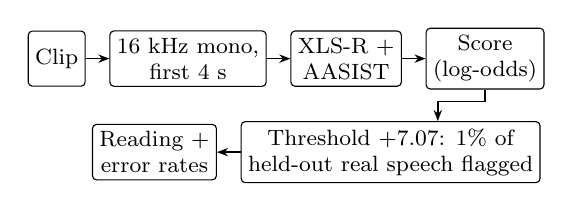
\begin{tikzpicture}[font=\footnotesize, node distance=3mm,
  box/.style={draw, rounded corners=1.5pt, align=center, inner sep=2.5pt,
              minimum height=7mm},
  arr/.style={-{Stealth[length=4pt]}, semithick}]
\node[box] (in) {Clip};
\node[box, right=of in] (pre) {16 kHz mono,\\first 4 s};
\node[box, right=of pre] (net) {XLS-R +\\AASIST};
\node[box, right=of net] (score) {Score\\(log-odds)};
\node[box, below=4mm of score, xshift=-12mm] (thr) {Threshold $+7.07$: 1\% of\\held-out real speech flagged};
\node[box, left=of thr] (out) {Reading +\\error rates};
\draw[arr] (in) -- (pre);
\draw[arr] (pre) -- (net);
\draw[arr] (net) -- (score);
\draw[arr] (score.south) -- ++(0,-1.5mm) -| ([xshift=6mm]thr.north);
\draw[arr] (thr) -- (out);
\end{tikzpicture}
\caption{The served pipeline. The score is compared with a threshold fitted
on held-out genuine speech and reported with the model's measured error
rates, not as a verdict.}
\label{fig:pipeline}
\end{figure}

\subsection{Training}
The CNN trains for five epochs (batch 64, Adam, learning rate $10^{-3}$);
AASIST follows its published recipe of 100 epochs (batch 24, $10^{-4}$, cosine
annealing), so the two differ by schedule as well as architecture. SSL-AASIST
uses the upstream recipe (batch 14, constant $10^{-6}$, weight decay
$10^{-4}$): 100 epochs on LA alone, or four epochs once SpeechFake is added
(about 12--13 hours on one H100). RawBoost (series algorithm~5) is applied to
training audio only. The private CNN uses DP-SGD with noise multiplier 1.1,
per-example clipping norm 1.0 and $\delta = 10^{-5}$, reaching
$\varepsilon = 0.48$ after five epochs. The checkpoint kept is the one with
the lowest development EER.

\subsection{Calibration and Reporting}
The model's two logits are reduced to one score, the log-odds of spoof; the
fine-tuned models saturate a float32 softmax, so probabilities near 1 cannot
be compared. The threshold is fitted on 10{,}000 genuine People's Speech clips
split by speaker: half to find the score that flags 1\% of them, half to check
it. For the served model this is $+7.07$ ($P = 0.99915$). The 95th percentile
of held-out genuine scores marks the start of an ``uncertain'' band below the
threshold. The application (Fig.~\ref{fig:ui}) reports the score on a scale
with the threshold and band drawn; a confidence derived from the distance to
the threshold, labelled as certainty rather than accuracy; and the served
model's error rates on each test set, read from evaluation reports measured
at the same threshold.

\begin{figure*}[!t]
\centering
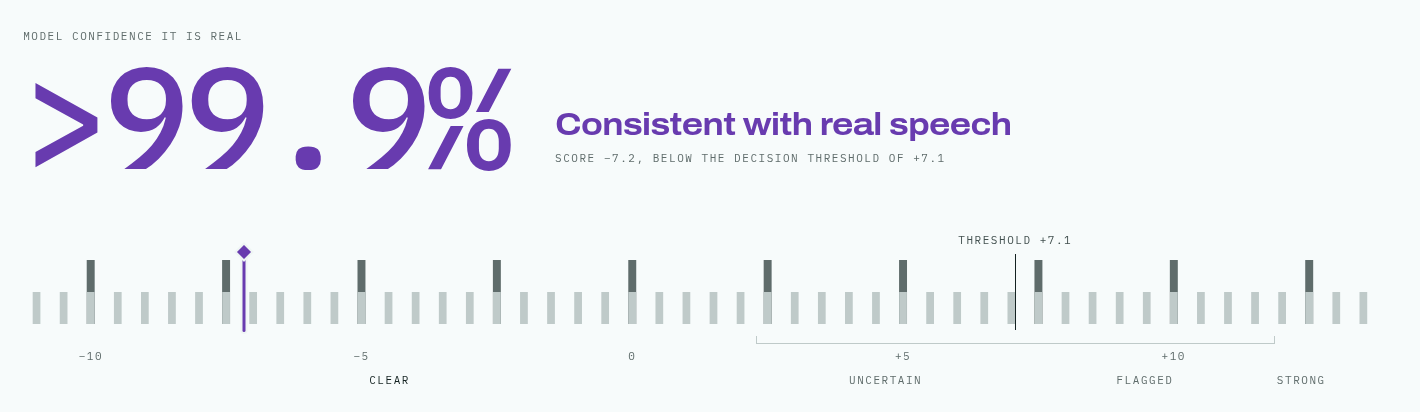
\includegraphics[width=0.82\textwidth]{figures/fig5_result.png}
\caption{A reading in the web application: a genuine clip scored $-7.2$
against the threshold of $+7.1$. The scale is the model's log-odds score,
with the uncertain band bracketed below it; the page continues with the
measured error rates of Table~\ref{tab:served}.}
\label{fig:ui}
\end{figure*}

\subsection{Evaluation Protocol}
We report EER and min t-DCF on evaluation partitions only, since LA's
development set reuses the training attacks; per-attack EER; and, at the
served threshold, the share of genuine clips flagged and of fakes missed, with
Wilson 95\% intervals~\cite{wilson1927}. From the tenth experiment on, each
was \emph{pre-registered}: the question, the single change, the outcome
categories and the serving criteria were written into the project's results
log before any job ran, and In-the-Wild was scored once per candidate. Twice
the project owner overrode a pre-registered bar; each override was written
down before the next job ran, and both are reported below.

% ===========================================================================
\section{Results}

\subsection{Benchmark Performance}
Table~\ref{tab:la} places our models among published ones. The CNN matches
the official baselines (10.15\% against 9.57\% and 8.09\%), and SSL-AASIST
with RawBoost reaches 0.79\% EER and 0.0143 min t-DCF, below published AASIST
on both. Our AASIST reaches 3.17\% against a published 0.83\%; candidate
causes are the GroupNorm substitution, a single seed and model selection,
since the checkpoint chosen by development EER ranks 23rd of 100 epochs on
evaluation. Selection by development EER also chose a worse CNN than an
earlier epoch: development EER fell to 0.24\% while evaluation EER stayed
near 10\%. Per attack, LFCC and log-Mel are complementary rather than ranked:
LFCC is better on nine of thirteen attacks, log-Mel on A18 and A19.

\begin{table}[!t]
\caption{ASVspoof 2019 LA evaluation partition. Published rows from the
cited papers; ours measured.}
\label{tab:la}
\centering
\footnotesize
\begin{tabular}{@{}lrr@{}}
\toprule
System & EER (\%) & min t-DCF \\
\midrule
CQCC-GMM (official baseline) & 9.57 & 0.2366 \\
LFCC-GMM (official baseline) & 8.09 & 0.2116 \\
AASIST (published)~\cite{jung2022aasist} & 0.83 & 0.0275 \\
\midrule
Ours: CNN, log-Mel & 10.15 & 0.2350 \\
Ours: CNN, log-Mel, DP ($\varepsilon = 0.48$) & 17.80 & 0.2696 \\
Ours: AASIST & 3.17 & 0.0909 \\
Ours: SSL-AASIST + RawBoost & 0.79 & 0.0143 \\
Ours: served model$^\dagger$ & 0.53 & 0.0173 \\
\bottomrule
\end{tabular}\\[2pt]
{\scriptsize $^\dagger$Not cleanly held out: SpeechFake shares VCTK with
LA's genuine speech.}
\end{table}

\subsection{The Cost of Privacy}
DP-SGD raised the CNN's evaluation EER from 10.15\% to 17.80\%, a cost of
7.65 points (7.97 comparing each regime's best epoch), and min t-DCF from
0.2350 to 0.2696. The cost is not spread evenly (Fig.~\ref{fig:dp}). The
private model is \emph{better} on A10--A15, below 0.7\% on each, worse on
A08 (0.83\% $\to$ 8.10\%), and close to chance on A17--A19 (43--45\%), where
the non-private model scores 41\%, 12\% and 3\%. Privacy noise did not blur the model uniformly; it removed two
attack families it had learned and left one it never had. Four caveats inflate
the gap: hyperparameters were not re-tuned for DP, $\varepsilon = 0.48$ is
far stricter than the $\varepsilon \approx 8$ common in DP deep learning,
training lasted five epochs, and there is one seed. Under noise the model's
development accuracy also sat at exactly the dataset's spoof share for all
five epochs, a warning that accuracy is meaningless on imbalanced data.

\begin{figure}[!t]
\centering
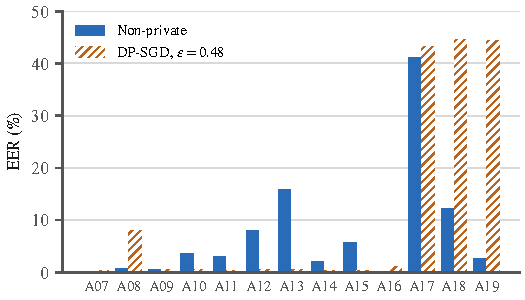
\includegraphics[width=\columnwidth]{figures/fig2_dp.pdf}
\caption{Per-attack EER on ASVspoof 2019 LA evaluation for the log-Mel CNN
with and without DP-SGD ($\varepsilon = 0.48$).}
\label{fig:dp}
\end{figure}

\begin{table*}[!t]
\caption{The served model at its threshold ($+7.07$), with Wilson 95\%
intervals. It was never trained, selected or calibrated on any of these sets.}
\label{tab:served}
\centering
\footnotesize
\begin{tabular}{@{}lL{6.2cm}rrr@{}}
\toprule
Test set & Contents & EER (\%) & Real flagged (\%) & Fakes missed (\%) \\
\midrule
In-the-Wild & real-world recordings and deepfakes of public figures & 2.02 & 2.18 (1.99--2.40) & 1.89 (1.66--2.15) \\
SpeechFake test (English) & clean modern TTS and voice conversion, 26 systems & 4.15 & 0.00 & 13.65 (13.50--13.81) \\
ASVspoof 2019 LA eval & clean studio speech, 2019-era attacks & 0.53 & 0.00 & 20.65 (20.34--20.97) \\
Own fakes, heldout-b & four open TTS families never heard & 7.70 & 3.51 (2.65--4.64) & 15.27 (14.19--16.42) \\
\bottomrule
\end{tabular}
\end{table*}

\subsection{Collapse and Recovery on Real-World Audio}
Fig.~\ref{fig:itw} follows In-the-Wild EER through the project. Every model
trained on LA alone failed: AASIST rose from 3.17\% on LA to 37.15\%, and the
CNN reached 58.54\%, ranking the classes the wrong way round. RawBoost made
AASIST \emph{worse} (48.78\%) while making it better on LA (1.74\%), and the
pre-trained front-end alone did nothing (37.86\%). Only the combination
worked: SSL-AASIST with RawBoost reached 11.21\%. A plausible reading is that
XLS-R already represents real speech well and RawBoost stops fine-tuning on
clean LA audio from overwriting that representation. Adding SpeechFake's 26
generators brought EER to 2.65\%, and our own eight TTS families to 2.02\%.
Adding genuine speech from Common Voice and VoxPopuli, by contrast, left the
ranking unchanged or slightly worse (2.71\%, 3.55\%).

\begin{figure}[!t]
\centering
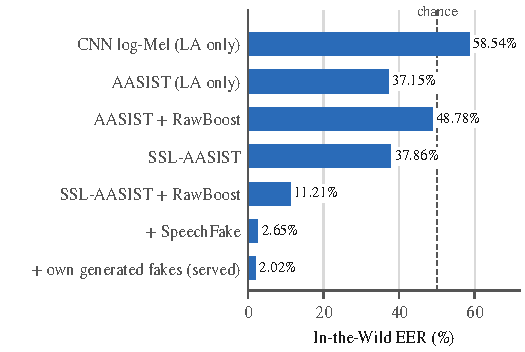
\includegraphics[width=\columnwidth]{figures/fig3_itw.pdf}
\caption{In-the-Wild EER of each model, in the order the experiments
produced them. Rows after ``SSL-AASIST + RawBoost'' add training data to it.
No model was trained, selected or calibrated on In-the-Wild.}
\label{fig:itw}
\end{figure}

\subsection{The Threshold}
Ranking was solved before the threshold was (Table~\ref{tab:thr}). At its
development-set threshold the 2.65\% model flagged most genuine In-the-Wild
clips. Calibrating on held-out real speech fixed this, but which real speech
mattered: training on Common Voice made Common Voice useless for calibrating,
and In-the-Wild's flagged rate rose to 53.7\%. Fitting on People's Speech, a
source the model never trained on, with a 1\% target transferred almost
exactly: 0.60\% flagged on the check half, 0.62\% on In-the-Wild, with 3.61\%
of fakes missed.

The cost appeared on clean audio. At that threshold 46.3\% of LA's fakes and
32.7\% of SpeechFake's passed, although 20 of SpeechFake's 26 systems had EERs
under 1.2\%: clean audio, genuine or fake, sits low on this model's scale,
and the threshold was set where noisy genuine speech sits. Three attempts to
reconcile the two failed against their pre-registered bars. Passing every
input through a fixed channel moved fakes down, not genuine speech up. A
second, stricter threshold for ``clean'' audio cut clean-fake misses by 9.6
points but sent 60.7\% of In-the-Wild's genuine clips down the clean route and
flagged 4.0\% of them. Augmenting training with random channels moved misses
by 2.0 points, against 10 required.

\begin{table}[!t]
\caption{Attempts to place one threshold for real-world and clean audio,
judged against criteria fixed before each run. ITW: In-the-Wild.}
\label{tab:thr}
\centering
\footnotesize
\begin{tabular}{@{}cL{3.0cm}L{3.5cm}@{}}
\toprule
\# & Change & Result \\
\midrule
10 & Common Voice as genuine training data & ITW real flagged 8.0\% $\to$ 53.7\%; worse \\
11 & + VoxPopuli; calibrate on People's Speech & 8.2\% $\to$ 8.9\%; no effect \\
12 & 1\% target on People's Speech & ITW 0.62\% flagged, 3.61\% missed; \textbf{served} \\
13 & Score clean modern fakes & 32.7\% of SpeechFake fakes pass \\
14 & Degrade every input & best candidate 4.1 points worse; not served \\
15 & Second threshold for clean audio & ITW real flagged 4.0\%; not served \\
16 & Random channel in training & misses $-2.0$ points, $-10$ needed; no effect \\
\bottomrule
\end{tabular}
\end{table}

\subsection{Training on Generated Fakes}
Before further training, the served model was scored on heldout-a: it let
88.5\% of these unheard TTS fakes through, and for Qwen3-TTS and VoxCPM its
EER was 39--45\%, near chance, so no threshold could have helped. We then
trained on 44{,}000 fakes from eight other open families. heldout-a misses fell
to 37.4\%, passing the gate, and every final test set improved
(Table~\ref{tab:served}): fakes missed fell by half or more everywhere, and
on heldout-b from 73.9\% to 15.3\%. The cost was on the genuine side. The same
1\% calibration now flagged 2.18\% of In-the-Wild's genuine clips, against a
pre-registered bar of 2\%, and 3.5\% of clean LibriSpeech. By its own criteria
the model was ``improved, not served''; the project owner overrode the
In-the-Wild bar and served it, a decision written down before the swap, on
the grounds that every other criterion passed by a wide margin. Qwen3-TTS and
VoxCPM still pass 64--84\% of the time. A final experiment would have
resynthesised genuine speech through two open neural codecs to teach the
model their fingerprint, but the served model already flagged 98--100\% of
it; these two systems evade the detector by some route other than a generic
codec signature.



% ===========================================================================
\section{Discussion}

\textbf{What generalised.} The result supports the claim behind
SSL-AASIST~\cite{tak2022ssl} and sharpens it: the pre-trained front-end was
necessary but not sufficient, and only generator diversity in training took
In-the-Wild from 11\% to 2\%. Genuine-speech diversity did not. This fits
M\"uller et al.'s diagnosis~\cite{muller2022itw} that benchmark models learn
the benchmark, and suggests that what they over-fit to is the fakes.

\textbf{One threshold, two kinds of audio.} Our central finding is the one
EER cannot show (Section~II-A): a model can rank both clean and noisy audio
well and still place them on different parts of its scale, so any single
threshold trades false accusations on noisy recordings against missed clean
fakes. The 1\% target makes that trade in favour of the person who might be
accused, which we judge right for a public tool, and the interface states the
consequence: a low reading on clean audio is not evidence of authenticity.

\textbf{Bias and error.} Every result is a single seed. The intervals in
Table~\ref{tab:served} cover clip sampling only, and In-the-Wild's clips share
54 speakers, so the true uncertainty is wider; the 2.18\% that missed its bar
has an interval of 1.99--2.40\%, so the miss is barely measurable. Model
selection used development sets that reuse training attacks; LA evaluation is
contaminated by VCTK once SpeechFake is used; and our own fakes, although
split by family, share LibriSpeech voices with the calibration check.
Pre-registration was our main control on researcher bias: In-the-Wild was
never consulted to choose anything, and failures were reported in the same
form as successes. Its limit is visible too: twice a bar was overridden, and
we can only report that, not undo it.

\textbf{Privacy.} One measurement on one small model is a point, not the
privacy--utility curve the question asks for. It does show that the cost
concentrates on particular attacks, so a pooled EER understates what a private
detector would miss. Because DP protects a public training set, the privacy a
user needs is at inference: the server keeps uploads in memory, never on disk,
and logs neither audio nor filenames.

\textbf{Reporting.} The interface answers the second half of the question by
design rather than by experiment: it shows the score, the threshold and the
measured error rates, and never a bare verdict. We did not test it with
users, so whether it reduces misplaced confidence remains a hypothesis.

% ===========================================================================
\section{Limitations and Future Work}
The detector reads only the first four seconds of a clip and does not verify
who is speaking. Recent LLM-based TTS with neural codecs (Qwen3-TTS, VoxCPM)
mostly passes, and clean genuine speech is now flagged more often (LibriSpeech
3.5\%). DP was measured only on the CNN, at one $\varepsilon$, with no private
AASIST or SSL-AASIST. Per-clip scores were not saved, so EER has no confidence
interval. Future work should score whole clips; retrain so that clean and
noisy audio share one scale; measure DP on SSL-AASIST with the front-end
frozen, across several values of $\varepsilon$; select models on a held-out
attack set; and test the interface with users.

\section{Conclusion}
A detector trained only on public data can work on real-world recordings: with
a pre-trained front-end, RawBoost and many generators in training, SSL-AASIST
reaches 2.02\% EER on In-the-Wild, flagging 2.18\% of genuine recordings and
missing 1.89\% of fakes at a threshold fitted on held-out real speech. The
harder problem was the threshold, because clean and noisy audio sit on
different parts of the model's scale; clean studio fakes are still missed
between one time in five and one in eight. A tool for the public should
therefore show its threshold and its measured errors, and say plainly that a
low score on a clean recording is not proof that it is real.

% ===========================================================================
\section*{Acknowledgment}
The authors thank Hui Cui for supervision, and the MASSIVE M3
cluster for compute (project df37; 228.7 GPU-hours). We thank the creators of
the datasets in Table~\ref{tab:data}, used under the licences listed there.

\section*{Use of Generative AI}
Claude (Anthropic) was used throughout the project: to write and debug code,
to orchestrate training and evaluation jobs on M3, to build the web
application, to draft the text of this paper, and to prepare its figures and
the presentation. The authors directed the work, checked every number against
the experiment logs, reviewed and edited all drafted text, and take full
responsibility for the content.

\section*{Author Contributions}
% Agreed 7 October 2026. Each member confirms his line before submission.
M.~M.~Khanzada led the project and developed the detector, the experiments
and their pre-registration, the evaluation and calibration, and the web
application and its hosting. A.~Muhammad wrote the first version of the front
end, restructured the repository, and reviewed and edited Sections II-A to
II-C and the references. F.~Mohammed reviewed and edited Sections II-D to II-G
and Figs.~\ref{fig:dp} and~\ref{fig:itw}. All authors prepared and delivered
the presentation.

\bibliographystyle{IEEEtran}
\bibliography{refs}

\end{document}
